\hypertarget{a00005}{
\section{Dokumentacja klasy ASS8.Klient.Form4}
\label{dd/dad/a00005}\index{ASS8::Klient::Form4@{ASS8::Klient::Form4}}
}
Klasa wyświetlająca okno do zmiany serwera.  


Diagram współpracy dla ASS8.Klient.Form4:\nopagebreak
\begin{figure}[H]
\begin{center}
\leavevmode
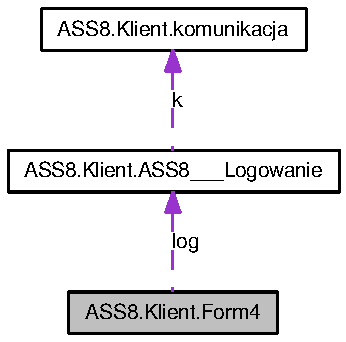
\includegraphics[width=202pt]{dc/de6/a00167}
\end{center}
\end{figure}
\subsection*{Metody publiczne}
\begin{CompactItemize}
\item 
\hyperlink{a00005_c9962a9d1b3f147eefe50994127df5d7}{Form4} (\hyperlink{a00001}{ASS8\_\-\_\-\_\-Logowanie} form)
\begin{CompactList}\small\item\em konstruktor klasy \item\end{CompactList}\end{CompactItemize}
\subsection*{Metody prywatne}
\begin{CompactItemize}
\item 
void \hyperlink{a00005_6683aa1b2eba62015b3a0abf81058a9c}{button1\_\-Click} (object sender, EventArgs e)
\begin{CompactList}\small\item\em Obsługa przycisku zapisz. \item\end{CompactList}\item 
void \hyperlink{a00005_a3ef6122bae46a2c4f90562b75b060b5}{button2\_\-Click} (object sender, EventArgs e)
\begin{CompactList}\small\item\em Obsługa przycisku zamknij. \item\end{CompactList}\end{CompactItemize}
\subsection*{Atrybuty prywatne}
\begin{CompactItemize}
\item 
\hyperlink{a00001}{ASS8\_\-\_\-\_\-Logowanie} \hyperlink{a00005_182469cf0d560d301c293d4961b44550}{log}
\end{CompactItemize}


\subsection{Opis szczegółowy}
Klasa wyświetlająca okno do zmiany serwera. 



Definicja w linii 14 pliku Form4.cs.

\subsection{Dokumentacja konstruktora i destruktora}
\hypertarget{a00005_c9962a9d1b3f147eefe50994127df5d7}{
\index{ASS8::Klient::Form4@{ASS8::Klient::Form4}!Form4@{Form4}}
\index{Form4@{Form4}!ASS8::Klient::Form4@{ASS8::Klient::Form4}}
\subsubsection[{Form4}]{\setlength{\rightskip}{0pt plus 5cm}ASS8.Klient.Form4.Form4 ({\bf ASS8\_\-\_\-\_\-Logowanie} {\em form})}}
\label{dd/dad/a00005_c9962a9d1b3f147eefe50994127df5d7}


konstruktor klasy 

\begin{Desc}
\item[Parametry:]
\begin{description}
\item[{\em form}]Formularz klasy wywołującej\end{description}
\end{Desc}


Definicja w linii 21 pliku Form4.cs.

\subsection{Dokumentacja funkcji składowych}
\hypertarget{a00005_6683aa1b2eba62015b3a0abf81058a9c}{
\index{ASS8::Klient::Form4@{ASS8::Klient::Form4}!button1\_\-Click@{button1\_\-Click}}
\index{button1\_\-Click@{button1\_\-Click}!ASS8::Klient::Form4@{ASS8::Klient::Form4}}
\subsubsection[{button1\_\-Click}]{\setlength{\rightskip}{0pt plus 5cm}void ASS8.Klient.Form4.button1\_\-Click (object {\em sender}, \/  EventArgs {\em e})\hspace{0.3cm}{\tt  \mbox{[}private\mbox{]}}}}
\label{dd/dad/a00005_6683aa1b2eba62015b3a0abf81058a9c}


Obsługa przycisku zapisz. 

\begin{Desc}
\item[Parametry:]
\begin{description}
\item[{\em sender}]\item[{\em e}]\end{description}
\end{Desc}


Definicja w linii 33 pliku Form4.cs.\hypertarget{a00005_a3ef6122bae46a2c4f90562b75b060b5}{
\index{ASS8::Klient::Form4@{ASS8::Klient::Form4}!button2\_\-Click@{button2\_\-Click}}
\index{button2\_\-Click@{button2\_\-Click}!ASS8::Klient::Form4@{ASS8::Klient::Form4}}
\subsubsection[{button2\_\-Click}]{\setlength{\rightskip}{0pt plus 5cm}void ASS8.Klient.Form4.button2\_\-Click (object {\em sender}, \/  EventArgs {\em e})\hspace{0.3cm}{\tt  \mbox{[}private\mbox{]}}}}
\label{dd/dad/a00005_a3ef6122bae46a2c4f90562b75b060b5}


Obsługa przycisku zamknij. 

\begin{Desc}
\item[Parametry:]
\begin{description}
\item[{\em sender}]\item[{\em e}]\end{description}
\end{Desc}


Definicja w linii 61 pliku Form4.cs.

\subsection{Dokumentacja atrybutów składowych}
\hypertarget{a00005_182469cf0d560d301c293d4961b44550}{
\index{ASS8::Klient::Form4@{ASS8::Klient::Form4}!log@{log}}
\index{log@{log}!ASS8::Klient::Form4@{ASS8::Klient::Form4}}
\subsubsection[{log}]{\setlength{\rightskip}{0pt plus 5cm}{\bf ASS8\_\-\_\-\_\-Logowanie} {\bf ASS8.Klient.Form4.log}\hspace{0.3cm}{\tt  \mbox{[}private\mbox{]}}}}
\label{dd/dad/a00005_182469cf0d560d301c293d4961b44550}




Definicja w linii 16 pliku Form4.cs.

Dokumentacja dla tej klasy została wygenerowana z pliku:\begin{CompactItemize}
\item 
\hyperlink{a00047}{Form4.cs}\end{CompactItemize}
